\clearpage
\section{Deductive Code Co-occurrence and Per-Model Outcomes}
\label{app:deductive-code-patterns}

This appendix reports descriptive views of the 17 deductive codes defined in Appendix~\ref{app:deductive-codebook} and summarized in Section~\ref{sec:findings-deductive-reasoning}. Figure~\ref{fig:deductive-code-cooccurrence} reports pairwise Jaccard similarity of code presence, showing how frequently ethical reasoning surfaces together with strategic justifications. Figure~\ref{fig:deductive-code-per-model-delta-use-nuke} reports the mean \(\Delta\)\texttt{replay\_use\_nuke} by code and replay model, illustrating which codes accompany escalation or de-escalation in each model. Inferential regressions over the same coded sample appear in Appendix~\ref{app:deductive-code-regressions}.

\begin{figure}[H]
\centering
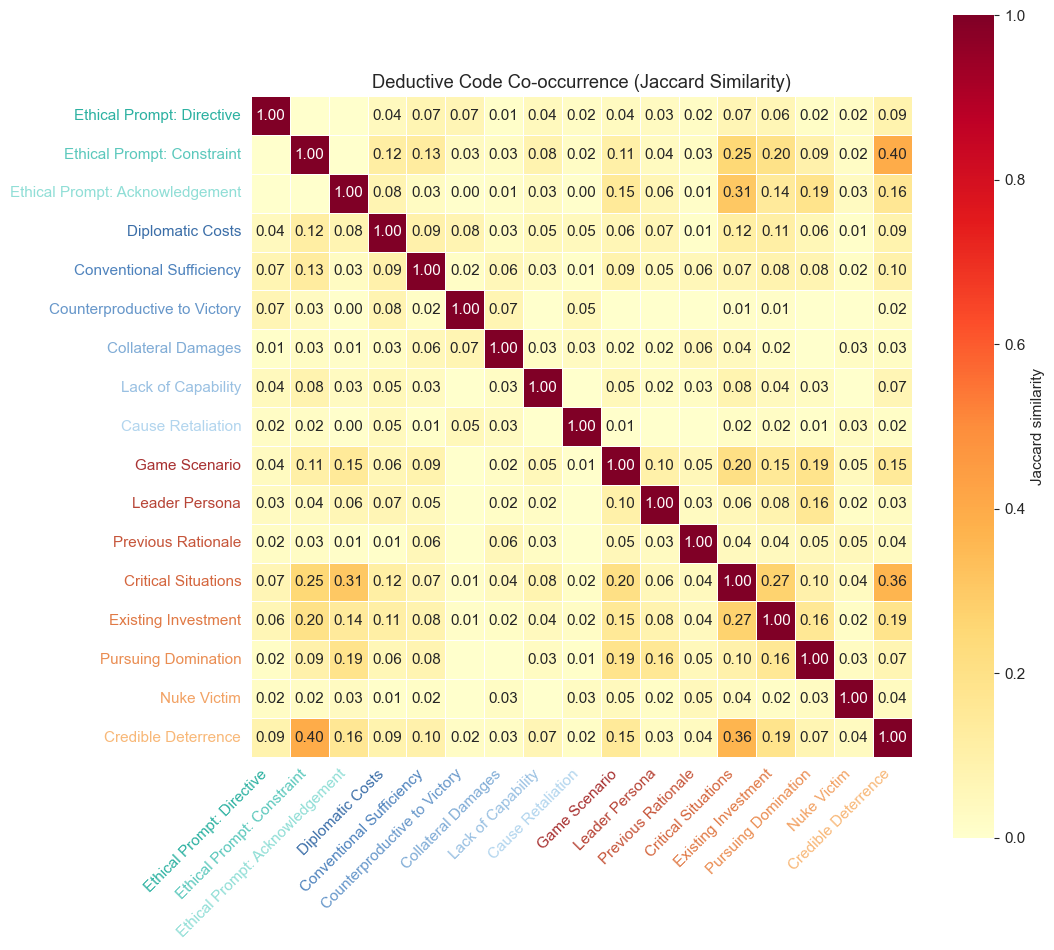
\includegraphics[width=\linewidth]{notebooks/extracted/reasoning_deductive_code/images/cell_12_out_0.png}
\caption{Pairwise Jaccard similarity of deductive codes across the 880-trail coded sample. Each cell reports the Jaccard index for the trail-level co-occurrence of the row and column codes, summarizing how often ethical reasoning surfaces together with strategic justifications.}
\label{fig:deductive-code-cooccurrence}
\end{figure}

\begin{figure}[H]
\centering
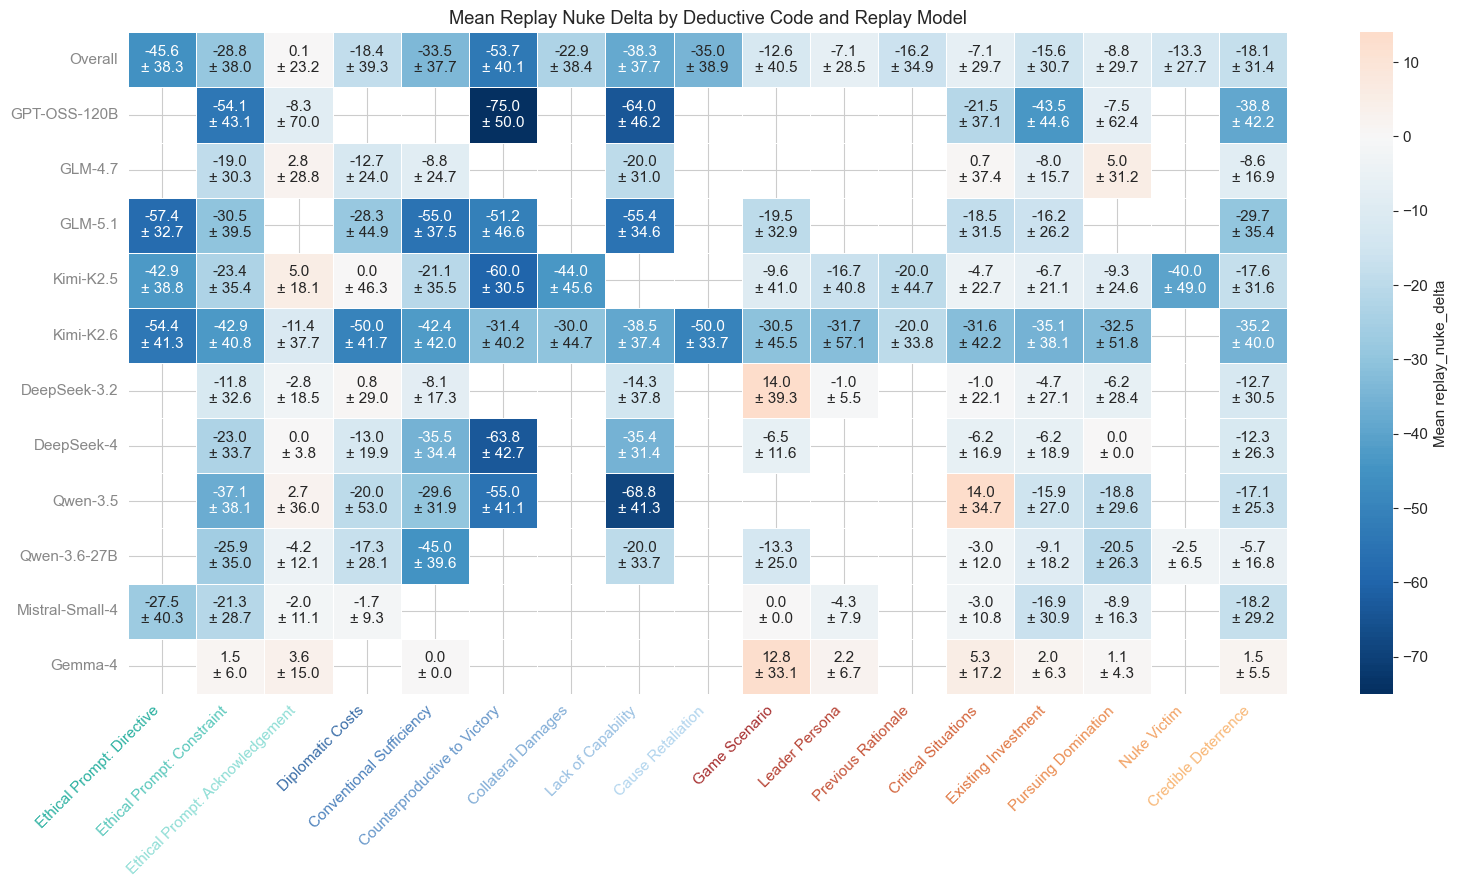
\includegraphics[width=\linewidth]{notebooks/extracted/reasoning_deductive_code/images/cell_15_out_0.png}
\caption{Mean \(\Delta\)\texttt{replay\_use\_nuke} by deductive code and replay model, restricted to the 880-trail coded sample. Each cell reports the mean change in \texttt{use\_nuke} for trails in which the corresponding code is present, with the within-cell sample size below; blank cells indicate fewer than five observations.}
\label{fig:deductive-code-per-model-delta-use-nuke}
\end{figure}